% ******************************* PhD Thesis Template **************************
% Please have a look at the README.md file for info on how to use the template

\documentclass[a4paper,12pt,times,numbered,print,index]{PhDThesisPSnPDF}

% ******************************************************************************
% ******************************* Class Options ********************************
% *********************** See README for more details **************************
% ******************************************************************************

% `a4paper'(The University of Cambridge PhD thesis guidelines recommends a page
% size a4 - default option) or `a5paper': A5 Paper size is also allowed as per
% the Cambridge University Engineering Deparment guidelines for PhD thesis
%
% `11pt' or `12pt'(default): Font Size 10pt is NOT recommended by the University
% guidelines
%
% `oneside' or `twoside'(default): Printing double side (twoside) or single
% side.
%
% `print': Use `print' for print version with appropriate margins and page
% layout. Leaving the options field blank will activate Online version.
%
% `index': For index at the end of the thesis
%
% `draftclassic': For draft mode without loading any images (same as draft in book)
%
% `draft': Special draft mode with line numbers, images, and water mark with
% timestamp and custom text. Position of the text can also be modified.
%
% `abstract': To generate only the title page and abstract page with
% dissertation title and name, to submit to the Student Registry
%
% `chapter`: This option enables only the specified chapter and it's references
%  Useful for review and corrections.
%
% ************************* Custom Page Margins ********************************
%
% `custommargin`: Use `custommargin' in options to activate custom page margins,
% which can be defined in the preamble.tex. Custom margin will override
% print/online margin setup.
%
% *********************** Choosing the Fonts in Class Options ******************
%
% `times' : Times font with math support. (The Cambridge University guidelines
% recommend using times)
%
% `fourier': Utopia Font with Fourier Math font (Font has to be installed)
%            It's a free font.
%
% `customfont': Use `customfont' option in the document class and load the
% package in the preamble.tex
%
% default or leave empty: `Latin Modern' font will be loaded.
%
% ********************** Choosing the Bibliography style ***********************
%
% `authoryear': For author-year citation eg., Krishna (2013)
%
% `numbered': (Default Option) For numbered and sorted citation e.g., [1,5,2]
%
% `custombib': Define your own bibliography style in the `preamble.tex' file.
%              `\RequirePackage[square, sort, numbers, authoryear]{natbib}'.
%              This can be also used to load biblatex instead of natbib
%              (See Preamble)
%
% **************************** Choosing the Page Style *************************
%
% `default (leave empty)': For Page Numbers in Header (Left Even, Right Odd) and
% Chapter Name in Header (Right Even) and Section Name (Left Odd). Blank Footer.
%
% `PageStyleI': Chapter Name next & Page Number on Even Side (Left Even).
% Section Name & Page Number in Header on Odd Side (Right Odd). Footer is empty.
%
% `PageStyleII': Chapter Name on Even Side (Left Even) in Header. Section Number
% and Section Name in Header on Odd Side (Right Odd). Page numbering in footer

% Uncomment to change page style
%\pagestyle{PageStyleII}

% ********************************** Preamble **********************************
% Preamble: Contains packages and user-defined commands and settings
% ******************************************************************************
% ****************************** Custom Margin *********************************

% Add `custommargin' in the document class options to use this section
% Set {innerside margin / outerside margin / topmargin / bottom margin}  and
% other page dimensions
\ifsetCustomMargin
  \RequirePackage[left=40mm,right=30mm,top=30mm,bottom=30mm]{geometry}
  \setFancyHdr % To apply fancy header after geometry package is loaded
\fi
\usepackage{pdfpages}
% Add spaces between paragraphs
%\setlength{\parskip}{0.5em}
% Ragged bottom avoids extra whitespaces between paragraphs
\raggedbottom
% To remove the excess top spacing for enumeration, list and description
%\usepackage{enumitem}
%\setlist[enumerate,itemize,description]{topsep=0em}

% *****************************************************************************
% ******************* Fonts (like different typewriter fonts etc.)*************

% Add `customfont' in the document class option to use this section

\ifsetCustomFont
  % Set your custom font here and use `customfont' in options. Leave empty to
  % load computer modern font (default LaTeX font).
  %\RequirePackage{helvet}

  % For use with XeLaTeX
  %  \setmainfont[
  %    Path              = ./libertine/opentype/,
  %    Extension         = .otf,
  %    UprightFont = LinLibertine_R,
  %    BoldFont = LinLibertine_RZ, % Linux Libertine O Regular Semibold
  %    ItalicFont = LinLibertine_RI,
  %    BoldItalicFont = LinLibertine_RZI, % Linux Libertine O Regular Semibold Italic
  %  ]
  %  {libertine}
  %  % load font from system font
  %  \newfontfamily\libertinesystemfont{Linux Libertine O}
\fi

% *****************************************************************************
% **************************** Custom Packages ********************************

% ************************* Algorithms and Pseudocode **************************

%\usepackage{algpseudocode}

\renewcommand{\chaptername}{CHAPTER}

\RequirePackage{titlesec}

\titleformat
{\chapter} % command
[display] % shape
{\bfseries\centering} % format
{\filcenter{\MakeUppercase{\chaptertitlename }} \thechapter} % label
{1pt} % sep
{
    \uppercase
} % before-code is code preceding the title body.
[
%\vspace{-0.5ex}%
%\rule{\textwidth}{0.3pt}
] % after-code is code following the title body.
%FORMAT ****** \titlespacing{<command>}{<left>}{<before-sep>}{<after-sep>} *****
\titlespacing{\chapter}{0pt}{0pt}{2ex}

\titleformat
{\section} % command
[hang] % shape
{\bfseries} % format
{\filright{\thesection}}  % label
{0pt} % sep
{
} % before-code is code preceding the title body.
\titlespacing{\section}{0pt}{10pt}{1pt}
%\titlespacing{\section}{0pt}{5.5ex plus 1ex minus .2ex}{4.3ex plus .2ex}

\titleformat
{\subsection} % command
[hang] % shape
{\bfseries} % format
{\filright{\thesubsection} } % label
{0pt} % sep
{
} % before-code is code preceding the title body.
\titlespacing{\subsection}{0pt}{10pt}{1pt}
%\titlespacing{\subsection}{0pt}{5.5ex plus 1ex minus .2ex}{4.3ex plus .2ex}

\titleformat
{\subsubsection} % command
[hang] % shape
{\bfseries} % format
{\filright{\thesubsubsection} } % label
{0pt} % sep
{
} % before-code is code preceding the title body.
\titlespacing{\subsubsection}{0pt}{10pt}{1pt}
%\titlespacing{\subsubsection}{0pt}{5.5ex plus 1ex minus .2ex}{4.3ex plus .2ex}

\usepackage[none]{hyphenat}

% ********************Captions and Hyperreferencing / URL **********************

% Captions: This makes captions of figures use a boldfaced small font.
%\RequirePackage[small,bf]{caption}

\RequirePackage[labelsep=space,tableposition=top]{caption}
\renewcommand{\figurename}{\textbf{Figure}} %to support older versions of captions.sty
\renewcommand{\tablename}{\textbf{Table}} %to support older versions of captions.sty

% *************************** Graphics and figures *****************************

%\usepackage{rotating}
%\usepackage{wrapfig}

% Uncomment the following two lines to force Latex to place the figure.
% Use [H] when including graphics. Note 'H' instead of 'h'
%\usepackage{float}
%\restylefloat{figure}

% Subcaption package is also available in the sty folder you can use that by
% uncommenting the following line
% This is for people stuck with older versions of texlive
%\usepackage{sty/caption/subcaption}
\usepackage{subcaption}

% ********************************** Tables ************************************
\usepackage{booktabs} % For professional looking tables
\usepackage{multirow}
\usepackage{adjustbox}
\usepackage{multicol}
\usepackage{longtable}
\usepackage{tabularx}
\usepackage{float}
\usepackage{colortbl}

% *********************************** SI Units *********************************
\usepackage{siunitx} % use this package module for SI units


% ******************************* Line Spacing *********************************

% Choose linespacing as appropriate. Default is one-half line spacing as per the
% University guidelines

% \doublespacing
% \onehalfspacing
% \singlespacing


% ************************ Formatting / Footnote *******************************

% Don't break enumeration (etc.) across pages in an ugly manner (default 10000)
%\clubpenalty=500
%\widowpenalty=500

%\usepackage[perpage]{footmisc} %Range of footnote options


% *****************************************************************************
% *************************** Bibliography  and References ********************

%\usepackage{cleveref} %Referencing without need to explicitly state fig /table

% Add `custombib' in the document class option to use this section
\ifuseCustomBib
   \RequirePackage[square, sort, numbers, authoryear]{natbib} % CustomBib


% If you would like to use biblatex for your reference management, as opposed to the default `natbibpackage` pass the option `custombib` in the document class. Comment out the previous line to make sure you don't load the natbib package. Uncomment the following lines and specify the location of references.bib file

% \RequirePackage[backend=biber, style=numeric-comp, citestyle=numeric, sorting=nty, natbib=true]{biblatex}
%\addbibresource{References/references} %Location of references.bib only for biblatex, Do not omit the .bib extension from the filename.

\fi

% changes the default name `Bibliography` -> `References'
\renewcommand{\bibname}{REFERENCES}


% ******************************************************************************
% ************************* User Defined Commands ******************************
% ******************************************************************************

% *********** To change the name of Table of Contents / LOF and LOT ************

%\renewcommand{\contentsname}{My Table of Contents}
%\renewcommand{\listfigurename}{My List of Figures}
%\renewcommand{\listtablename}{My List of Tables}


% ********************** TOC depth and numbering depth *************************

\setcounter{secnumdepth}{2}
\setcounter{tocdepth}{2}


% ******************************* Nomenclature *********************************

% To change the name of the Nomenclature section, uncomment the following line

%\renewcommand{\nomname}{Symbols}


% ********************************* Appendix ***********************************

% The default value of both \appendixtocname and \appendixpagename is `Appendices'. These names can all be changed via:

%\renewcommand{\appendixtocname}{List of appendices}
%\renewcommand{\appendixname}{Appndx}

% *********************** Configure Draft Mode **********************************

% Uncomment to disable figures in `draft'
%\setkeys{Gin}{draft=true}  % set draft to false to enable figures in `draft'

% These options are active only during the draft mode
% Default text is "Draft"
%\SetDraftText{DRAFT}

% Default Watermark location is top. Location (top/bottom)
%\SetDraftWMPosition{bottom}

% Draft Version - default is v1.0
%\SetDraftVersion{v1.1}

% Draft Text grayscale value (should be between 0-black and 1-white)
% Default value is 0.75
%\SetDraftGrayScale{0.8}


% ******************************** Todo Notes **********************************
%% Uncomment the following lines to have todonotes.

%\ifsetDraft
%	\usepackage[colorinlistoftodos]{todonotes}
%	\newcommand{\mynote}[1]{\todo[author=kks32,size=\small,inline,color=green!40]{#1}}
%\else
%	\newcommand{\mynote}[1]{}
%	\newcommand{\listoftodos}{}
%\fi

% Example todo: \mynote{Hey! I have a note}

% ******************************** Highlighting Changes **********************************
%% Uncomment the following lines to be able to highlight text/modifications.
%\ifsetDraft
%  \usepackage{color, soul}
%  \newcommand{\hlc}[2][yellow]{{\sethlcolor{#1} \hl{#2}}}
%  \newcommand{\hlfix}[2]{\texthl{#1}\todo{#2}}
%\else
%  \newcommand{\hlc}[2]{}
%  \newcommand{\hlfix}[2]{}
%\fi

% Example highlight 1: \hlc{Text to be highlighted}
% Example highlight 2: \hlc[green]{Text to be highlighted in green colour}
% Example highlight 3: \hlfix{Original Text}{Fixed Text}

% *****************************************************************************
% ******************* Better enumeration my MB*************
\usepackage{enumitem}


% ************************ Thesis Information & Meta-data **********************
% Thesis title and author information, refernce file for biblatex
% ************************ Thesis Information & Meta-data **********************
%% The title of the thesis
\title{Writing your PhD thesis in \texorpdfstring{\\ \LaTeX2e}{LaTeX2e}}
%\texorpdfstring is used for PDF metadata. Usage:
%\texorpdfstring{LaTeX_Version}{PDF Version (non-latex)} eg.,
%\texorpdfstring{$sigma$}{sigma}

%% Subtitle (Optional)
\subtitle{Using the CUED template}

%% The full name of the author
\author{Evianita Dewi Fajrianti}

%% Department (eg. Department of Engineering, Maths, Physics)
\dept{Department of Electrical Engineering}

%% University and Crest
\university{Politeknik Elektronika Negeri Surabaya}
% Crest minimum should be 30mm.
\crest{\includegraphics[width=0.2\textwidth]{University_Crest}}
%% Use this crest, if you are using the college crest
%% Crest long miminum should be 65mm
%\crest{\includegraphics[width=0.45\textwidth]{University_Crest_Long}}

%% College shield [optional] 
% Crest minimum should be 30mm.
%\collegeshield{\includegraphics[width=0.2\textwidth]{CollegeShields/Kings}}


%% Supervisor (optional)
%% for multiple supervisors, append each supervisor with the \newline command
%\supervisor{Prof. A.B. Supervisor\newline
%Prof. C.D. Supervisor}

%% Supervisor Role (optional) - Supervisor (default) or advisor
% \supervisorrole{\textbf{Supervisors: }}
%% if no title is desired:
% \supervisorrole{}

%% Supervisor line width: required to align supervisors
%\supervisorlinewidth{0.35\textwidth}

%% Advisor (optional)
%% for multiple advisors, append each advisor with the \newline command
%\advisor{Dr. A. Advisor\newline
%Dr. B. Advisor}
     
%% Advisor Role (optional) - Advisor (default) or leave empty
% \advisorrole{Advisors: }
%% if no title is required
% \advisorrole{}

%% Advisor line width: required to align supervisors
%\advisorlinewidth{0.25\textwidth}


%% You can redefine the submission text:
% Default as per the University guidelines:
% ``This dissertation is submitted for the degree of''
%\renewcommand{\submissiontext}{change the default text here if needed}

%% Full title of the Degree
\degreetitle{Doctor of Philosophy}

%% College affiliation (optional)
\college{King's College}

%% Submission date
% Default is set as {\monthname[\the\month]\space\the\year}
%\degreedate{September 2014} 

%% Meta information
\subject{LaTeX} \keywords{{LaTeX} {PhD Thesis} {Engineering} {University of
Cambridge}}


% ***************************** Abstract Separate ******************************
% To printout only the titlepage and the abstract with the PhD title and the
% author name for submission to the Student Registry, use the `abstract' option in
% the document class.

\ifdefineAbstract
 \pagestyle{empty}
 \includeonly{Declaration/declaration, Abstract/abstract}
\fi

% ***************************** Chapter Mode ***********************************
% The chapter mode allows user to only print particular chapters with references
% Title, Contents, Frontmatter are disabled by default
% Useful option to review a particular chapter or to send it to supervisior.
% To use choose `chapter' option in the document class

\ifdefineChapter
 \includeonly{Chapter3/chapter3}
\fi

% ******************************** Front Matter ********************************
\begin{document}

\frontmatter

% \maketitle

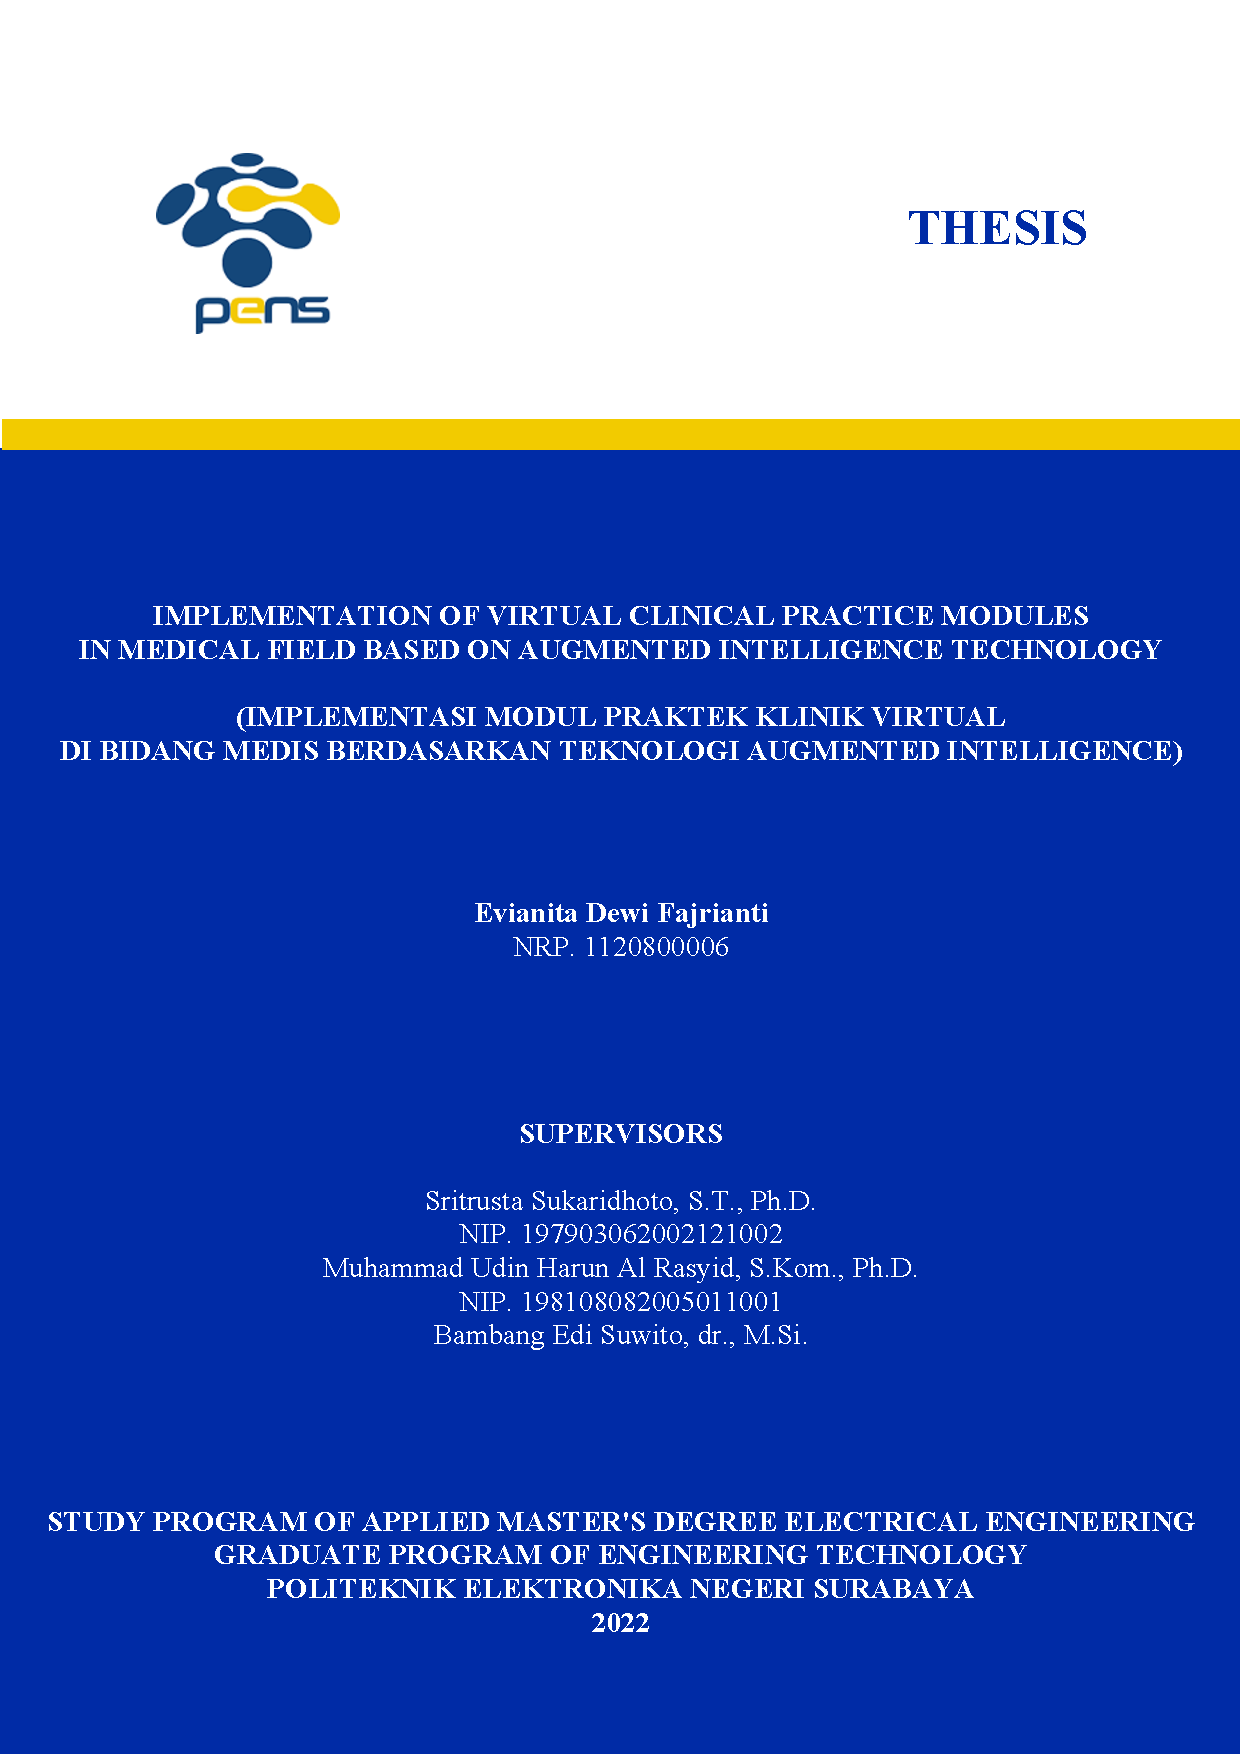
\includepdf{cover.pdf}
\begin{preface}
    
First of all, In the Name of Allah, the Most Gracious, the Most Merciful First of all the author's deepest thank To Allah SWT, the lord of the universe and to our prophet Muhammad SAW, may peace and blessing be upon him, his family and his followers., writer finished writing the thesis entitled 

\textbf{“IMPLEMENTATION OF VIRTUAL CLINICAL PRACTICE MODULES
IN MEDICAL FIELD BASED ON AUGMENTED INTELLIGENCE TECHNOLOGY” }
\textbf{
“IMPLEMENTASI MODUL PRAKTEK KLINIK VIRTUAL
DI BIDANG MEDIS BERDASARKAN TEKNOLOGI AUGMENTED INTELLIGENCE”}

Right in the calculated time.

The purpose in writing this thesis is to fulfil the assignment that given by PENS Graduate School as the requirement to finish the Master Degree in Electrical Engineering major. 

In arranging this paper, the writer truly get lots of challenges and obstructions but with help of many individuals, those obstructions could pass. Writer also realized there are still many mistakes in process of writing this thesis report. Because of that, the writer says thank you to all individuals who helps in the process of writing this paper. Hopefully Allah replies all helps and bless you all. The writer realized that this thesis report still imperfect in arrangement and the content.  Then the writer hopes the criticism from the readers can help the writer in perfecting the next research. Last but not the least hopefully, this thesis can help the readers to gain more knowledge about Augmented Intelligence.


\end{preface}
% ******************************* Thesis Dedidcation ********************************

\begin{dedication} 

I would like to dedicate this thesis to my loving parents and my homely family \dots

\end{dedication}


\include{Pengesahan/pengesahan.tex}

% ************************** Thesis Acknowledgements **************************

\begin{acknowledgements}      

\noindent This research was supported by Politeknik Elektronika Negeri Surabaya (PENS) -
Indonesia through Program Riset Keilmuan Terapan organized by Direktorat Jenderal Pendidikan Vokasi, Kementerian Pendidikan, Kebudayaan, Riset, dan Teknologi (Kemendikbudristek). 
With funding through Lembaga Pengelola Dana Pendidikan (LPDP). 
\begin{table}[h!]
    \centering
    \resizebox{15cm}{!}{%
    \begin{tabular}{p{0.2\linewidth}p{0.01\linewidth}p{0.7\linewidth}}
        Contract numbers & : & 0761/D6/KU.04.00/2021 \\
        Title & : & Implementasi Learning Management System Berbasis Virtual Reality Terintegrasi sebagai Media Pembelajaran untuk Meningkatkan Keterampilan Siswa Vokasi dalam Rangka Mendukung Program Merdeka Belajar Kampus Merdeka.\\
        Lead researcher & : & Sritrusta Sukaridhoto, S.T., Ph.D.\\
        Members & : & Muhammad Udin Harun Al Rasyid, S.Kom., Ph.D.\\
        &  & Ilham Achmad Al Hafidz, S.Tr.T.\\
        &  & Evianita Dewi Fajrianti, S.Tr.T. \\
        &  & Kirana Hanifa\\
        &  & Ita Zoeriah, SE.\\
    \end{tabular}}
\end{table}\\
This research was also supported by Universitas Nahdlatul Ulama Surabaya (UNUSA) -
Indonesia under contract Scheme 6 Numbers:
161.6.5/UNUSA/Adm-LPPM/III/2021.



\end{acknowledgements}

% ******************************* Thesis Declaration ***************************

\begin{declaration}

I hereby declare that part or all of this thesis:

\begin{enumerate}
    \item Is the result of own work and does not contain elements of plagiarism from other parties
    \item  Has never been submitted for an academic degree at a university
    \item Never or written by another party
    \item References and quotes honestly and correctly to other reference sources that support the discussion in the thesis.
\end{enumerate}


If the evidence that my statement is not true, then I will receive a sanction by the applicable provisions at the Politeknik Elektronika Negeri Surabaya.

% Author and date will be inserted automatically from thesis.tex \author \degreedate

\end{declaration}


\begin{publication}
For the sake of scientific development, I hereby declare:

\begin{enumerate}
    \item give approval to the Politeknik Elektronika Negeri Surabaya to store, the process in the form of data, maintain, transfer media/format and publish this thesis as long as my name remains as the author/creator and as the owner of the Copyright.
    \item not to transfer media/formats and publications in the form of scientific papers from parts or the whole of this thesis to a scientific publication, in seminars or journals, on a national or international scale, unless there is approval from me and the Main Advisory Lecturer, and propose my name, Lecturer Principal Advisor and other names (if any) who contributed to the paper.
\end{enumerate}


\end{publication}
% ************************** Thesis Acknowledgements **************************

\begin{thankyou}      
On this occasion the author would like to express deepest gratitude to several parties who have provided support during the process of completing this Final Thesis, including:

\begin{enumerate}
    \item The author's parents, Nurul Huda and Handayani, author's sister Rizka Amelia Rohmah, SE., M.MT., and author's husband Amma Liesvarastranta Haz, S.Tr.T.  as well as the entire extended family always send prayers, encouragement, advice, understanding, and great patience in guiding me.
    \item Mr. Sritrusta Sukaridhoto, S.T., Ph.D. and Mr. Muhammad Udin Harun Al Rasyid, S. Kom., Ph.D. as a thesis supervisor who has helped, financed, and guided so that this report can be completed. Without them, I'm just an ordinary student who works every day without direction and purpose.
    \item Mrs. Dr.Ing Hestiasari Rante, ST., M.Sc, Mr. Dr.Eng. Indra Adji Sulistijono, ST, M.Eng., and Mr. Reesa Akbar, ST., MT., Ph.D. As a Final Thesis examiner who has provided suggestions to the author.
    %item Bapak Dr.Eng. Indra Adji Sulistijono, ST, M.Eng., Bapak Didik Setyo Purnomo, S.T., M.Eng., dan Ibu Zaqiatud Darojah, S.Si., M.Si. Selaku penguji Proyek Akhir yang telah memberikan saran dan masukan kepada penulis.
    \item Mrs. Rizqi Putri Nourma Budiarti, S.T., M.T. and Mr. Bambang Edi Suwito, dr., M.Si. as a supervisor as well as a validator in the medical field, also providing adequate assets and equipment while working on a thesis at the Virtual Reality Lab. - UNUSA.
    \item All Mr and Mrs lecturers in the EEPIS Postgraduate Program, especially the Department of Electrical Engineering, who have provided knowledge, advice, and are sincere all this time.
    %\item Bapak Muhammad Gatut Hermandana, Bapak Muhammad Nugraha Akbar, A.Md., Bapak Yasin Setio Budi, A.Md., dan Bapak Erwin Ardiansyah, A.Md., yang telah membantu dan memberi dukungan moril selama ini.
    \item The residents of Human Centric Multimedia Lab. PS.09.02 and Virtual Reality Lab. - UNUSA, especially my friends in the Immersive team, Ilham Achmad Al Hafidz, Naufal Adi Satrio, Luqmanul Hakim Iksan, and Ardiman Firmanda, are fighting together for their respective dreams.
    %\item Teman-teman D4 Teknik Mekatronika 2016 yang selalu menginspirasi dan menyemangati. Terutama untuk Kerent, Ardian, SKS, Adif, Amma, Faris, Satriya, Ircham, Alif, Dion, Agus, Bos Janto, Khoifan, Najeb, dan Diba yang selalu membuat kelucuan di kontrakan.
    %\item Teman-teman klaster kontrakan Damai II 35 yang menyediakan tempat berkeluh kesah selama pandemi.
    \item And all parties who have helped in the implementation of the thesis are not mentioned one by one.
\end{enumerate} 

In preparing this thesis report, the author is aware of the shortcomings in both the preparation and discussion of the problem due to the author's limited knowledge. For this reason, the author expects constructive criticism and suggestions from all parties so that it can be better in the future. Thank you.




\end{thankyou}

% ************************** Thesis Abstract *****************************
% Use `abstract' as an option in the document class to print only the titlepage and the abstract.
\begin{abstract}
People's skills are getting better as technology advances, which is in line with the fact that education is getting better day by day. One way is through augmented intelligence, where humans and technology work together to make people smarter. In this study, augmented intelligence is used to help people learn about human anatomy. This is done by using augmented reality technology to track motion, which can make 3D objects follow the motion. The platform for studying anatomy is called AIVE (Artificial Intelligence in Virtual Education).


\end{abstract}

\begin{abstrak}
    Keterampilan masyarakat semakin baik seiring dengan kemajuan teknologi, yang sejalan dengan kenyataan bahwa pendidikan semakin hari semakin baik. Salah satu caranya adalah melalui augmented intelligence, di mana manusia dan teknologi bekerja sama untuk membuat orang menjadi lebih pintar. Dalam penelitian ini, augmented intelligence digunakan untuk membantu orang belajar tentang anatomi manusia. Hal ini dilakukan dengan menggunakan teknologi augmented reality untuk melacak gerakan, yang dapat membuat objek 3D mengikuti gerakan. Platform untuk mempelajari anatomi disebut AIVE (Kecerdasan Buatan dalam Pendidikan Virtual). $\phi*\psi=g+opo 0.123{00303}$

Penelitian ini dibagi menjadi 3 mode utama, yaitu mode studi, mode ujian, dan mode pelacakan gerakan manusia. Setiap mode dapat dioperasikan melalui tombol yang 
\end{abstrak}

% *********************** Adding TOC and List of Figures ***********************

\tableofcontents

\listoffigures

\listoftables

% \printnomenclature[space] space can be set as 2em between symbol and description
%\printnomenclature[3em]

\printnomenclature

% ******************************** Main Matter *********************************
\mainmatter

%!TEX root = ../thesis.tex
%*******************************************************************************
%*********************************** First Chapter *****************************
%*******************************************************************************

\chapter{INTRODUCTION}  %Title of the First Chapter

\ifpdf
    \graphicspath{{Chapter1/Figs/Raster/}{Chapter1/Figs/PDF/}{Chapter1/Figs/}}
\else
    \graphicspath{{Chapter1/Figs/Vector/}{Chapter1/Figs/}}
\fi


%********************************** %First Section  **************************************
\section{Background} %Section - 1.1 
Deskripsikan latar belakang dari permasalahan yang akan diangkat pada penelitian tesis. Latar belakang berisi penjelasan dari Problem Domain yang termuat pada  judul  penelitian. Misalkan penulis mengambil suatu judul berikut "Deteksi Penyakit Kanker Dengan Sistem Pakar Berbasis Fuzzy". Judul tersebut mempunyai Problem adalah Deteksi Penyakit Kanker, Problem Domain adalah Penyakit Kanker, dan Uniqueness adalah Sistem Pakar Berbasis Fuzzy.
Berkaitan dengan Latar Belakang, Problem Domain-nya adalah tentang penyakit kanker, sehingga disini penulis dapat menceritakan tentang penyakit kanker dan tingkat urgensi (seperti tingkat kenaikan jumlah penderitanya dari tahun ke tahun, gawatnya penyakit kanker tersebut, dan semisalnya). Latar belakang yang baik berisikan problem domain yang mempunyai tingkat urgensi tinggi.


% Please add the following required packages to your document preamble:
% \usepackage{graphicx}
\begin{table}[h!]
\centering
\caption{Comparison Between Virtual Reality With Augmented Reality.}
\label{table:vrar}
\resizebox{15cm}{!}{%
\begin{tabular}{|p{0.2\linewidth}|p{0.45\linewidth}|p{0.45\linewidth}|}\hline
Difference &
  AR &
  VR \\\hline
Environment &
  Combining   the real and virtual worlds. Thus, objects that coexist in the same space and   real-time are a reality. &
  VR environment requires an immersive virtual world environment that   replaces the real world. \\\hline
User Views &
  Allows   the user to see the real world around him and virtual objects &
  Users only see the virtual environment \\\hline
Health Point of View &
  AR solves the problem of "motion   sickness" through superimposing virtual images in a real environment   through special markers where the human brain is still able to process and   accept ideas &
  Known as "motion sickness- where the   human brain cannot distinguish between virtual and real and causes nausea and   severe headaches when adapting \\\hline
Security &
  The user feels comfortable and able to   control the environment. &
  Users feel uncomfortable because their view   is blocked by the virtual environment \\\hline
Immersion Sensation &
  None - Low &
  Medium   - High\\\hline
\end{tabular}%
}
\end{table}


Augmented Reality was chosen with the following considerations, which can be seen in the Table \ref{table:vrar}. This module is embedded in an application with a choice of operating systems iOS and Android \cite{Majid2015}. The difference lies in the addition of a control close loop that allows real-time reading of data which can then update parameters to generate new insights quickly. Based on the explanation in Table \ref{table:vrar}. 

\section{Research Problems}
Deskripsikan dengan jelas permasalahan yang ingin diteliti pada tesis. Permasalahan berisi penjelasan dari Problem yang termuat pada judul penelitian. Deskripsi masalah sebaiknya dituliskan dengan gaya bahasa deskriptif. Pada contoh judul diatas, Problem-nya adalah tentang deteksi penyakit kanker, sehingga penulis disini dapat menceritakan tentang sulitnya pendeteksian penyakit kanker dengan mendeskripsikan faktor-faktor yang membuat sulit dalam pendeteksiannya. Uraian permasalahan yang baik manakala penulis berhasil menyakinkan kepada pembaca tentang seberapa tingkat urgensi dari permasalahan tersebut sehingga membuat pembaca yakin bahwa permasalahan tersebut membutuhkan solusi dari penelitian pada tesis penulis.
\section{Contribution}
The contribution of this research to the medical field, especially medical and nursing students
\begin{enumerate}
    \item Using augmented intelligence technology, facilitate students' understanding of the structure of human anatomy.
    \item Presenting interactive and interesting learning concepts to reduce boredom during practicum.
    \item Provide self-training for students to study and test their abilities through quiz mode and learning mode.
\end{enumerate}
The contribution of this research for researchers, especially in the field of immersive technology
\begin{enumerate}
    \item The use of AR technology can be applied in the medical field while still taking into account the dependencies of human health.
    \item As a guide for the application of Augmented Intelligence technology that can show human movements through embedded artificial intelligence.
    \item Provides insight into building a good user experience by measuring system performance through the PIECES framework.
\end{enumerate}
The contribution of this research for users outside the end-user
\begin{enumerate}
    \item As a means of entertainment in the field of Augmented Reality technology.
    \item As a means of exploration for users to learn independently of the structure of human anatomy.
     \item As a means of information AR technology can be implemented in various fields, not only as a game but also as a learning tool.
\end{enumerate}

\section{Aims}
Deskripsikan dengan jelas tujuan penelitian tesis yang diangkat. Tujuan tesis harus jelas, singkat, dan mengandung klaim orisinalitas. Tuliskan secara argumentatif apa saja fitur-fitur yang ditawarkan pada penelitian sebagai sesuatu solusi yang baru untuk mengklaim orisinalitas pada penelitian tesis. Untuk memberikan gambaran yang jelas apa yang dilakukan dan solusi unik apa yang akan ditawarkan pada penelitian, tujuan sebaiknya diawali dengan kalimat pembuka seperti ini: “Penelitian tesis ini mengajukan suatu pendekatan / algoritma / pemodelan / teknik / metode yang baru untuk mengatasi ........................ (hubungan dengan Problem) dengan memakai / menggunakan / mempresentasikan / melibatkan ..................... (sebutkan solusi memakai apa)”. Kalimat-kalimat selanjutnya kemudian memperjelas solusi dengan fitur-fitur unik seperti apa yang ditawarkan pada penelitian sebagai suatu solusi untuk menjawab permasalahan.
Pada contoh judul diatas, orisinalitasnya adalah Sistem Pakar Berbasis Fuzzy, sehingga penulis disini dapat menjelaskan tentang pemodelan sistem pakar dan fitur-fitur fuzzy yang seperti apa untuk deteksi penyakit kanker. Kalimat pertama pada tujuan dapat diawali dengan contoh berikut, “Penelitian tesis ini mengajukan suatu pendekatan baru untuk pendeteksian penyakit kanker dengan mempresentasikan model klasifikasi menggunakan Sistem Pakar yang berbasis Fuzzy”. Kemudian pada kalimat-kalimat berikutnya terangkan secara argumentatif tentang fitur-fitur unik pemodelan Sistem Pakar dengan Fuzzy sehingga dapat digunakan untuk mendeteksi penyakit kanker.

The aims of this research are:{\vspace{-2ex}}
\begin{enumerate}
       \item Create a clinical practice module using Augmented Intelligence technology installed on mobile devices.{\vspace{-2ex}}
       \item Implements healthcare scenarios into clinical practice modules for multiple operating system options. {\vspace{-2ex}}
       \item Implemented the facial anatomy structure selection feature on mobile devices.{\vspace{-2ex}}
       \item Analyzes changes in facial movements that can interact with visual and non-visual sensors to transmit data on the mobile device display.{\vspace{-2ex}}
\end{enumerate}

\section{Advantage}
Uraikan kontribusi tesis pada pengembangan ilmu pengetahuan teknologi dan seni, pemecahan masalah pembangunan, atau pengembangan kelembagaan. Kontribusi menggambarkan manfaat dari penelitian terhadap pihak tertentu saat penelitian sudah selesai. Kontribusi sebaiknya bersifat spesifik, tidak terlalu luas dan tidak terkesan mengada-ada. Jelaskan siapa yang mendapatkan manfaat dari penelitian penulis dan dalam bentuk apa manfaatnya.

\section{Writing System}

Jelaskan tentang sistematika pembahasan dalam buku tesis yang meliputi:
\\
CHAPTER 1 INTRODUCTION

Jelaskan tentang apa saja yang dibahas pada Bab 1. Penjelasan memuat bagian-bagian penting pada Pendahuluan.
\\
CHAPTER 2: LITERATURE STUDY

Jelaskan tentang apa saja yang dibahas pada Bab 2. Penjelasan memuat bagian-bagian penting pada Kajian Pustaka.
\\
CHAPTER 3: SYSTEM DESIGN AND DEVELOPMENT

Jelaskan tentang apa saja yang dibahas pada Bab 3. Penjelasan memuat bagian-bagian penting pada Desain Sistem.
\\
CHAPTER 4: SYSTEM TESTING AND ANALYSIS

Jelaskan tentang apa saja yang dibahas pada Bab 4. Penjelasan memuat bagian-bagian penting pada Eksperimen dan Analisis.
\\
CHAPTER 5: CONCLUSION

Jelaskan tentang apa saja yang dibahas pada Bab 5. Penjelasan memuat bagian-bagian penting pada Penutup.

\nomenclature[z-AIVE]{AIVE}{Artificial Intelligence in Virtual Education}
\nomenclature[z-SLAM]{SLAM}{Simultaneous Localization and Mapping}
\nomenclature[z-IMU]{IMU}{Inertia Measurement Unit}
\nomenclature[z-AR]{AR}{Augmented Reality}
\nomenclature[z-VR]{VR}{Virtual Reality}
\nomenclature[z-AI]{AI}{Artifical Inteligence}
\nomenclature[s-AuI]{AuI}{Augmented Intelligence}
\nomenclature[z-UI]{UI}{User Interface}

%!TEX root = ../thesis.tex
%*******************************************************************************
%****************************** Second Chapter *********************************
%*******************************************************************************

\chapter{LITERATURE REVIEW}

\ifpdf
    \graphicspath{{Chapter2/Figs/Raster/}{Chapter2/Figs/PDF/}{Chapter2/Figs/}}
\else
    \graphicspath{{Chapter2/Figs/Vector/}{Chapter2/Figs/}}
\fi

Awali pembahasan pada bab ini dengan mengutarakan Problem pada Problem Domain dari tesis. Setelah itu, penjelasan tersebut diiringi dengan teori-teori penunjang pada bidang  pengetahuan yang terkait dengan Problem Domain dan Problem. Untuk lebih menguatkan klaim orisinalitas tesis penulis, perlu diberikan ulasan tentang penelitian-penelitian terkait yang juga bertujuan untuk mencoba menyelesaikan Problem tersebut. 

\section{Supporting Theory}
Uraikan dengan jelas dasar teori yang menunjang penelitian tesis yang akan dilakukan. Teori penunjang menguraikan dasar-dasar teori, temuan, dan bahan  dari pustaka ilmiah lain, yang dijadikan landasan untuk melakukan tesis yang diusulkan. Uraian dalam Teori Penunjang menjadi landasan untuk menyusun kerangka atau konsep yang akan digunakan dalam tesis.
\subsection{Augmented Intelligence in Industry 4.0}
The concept of Augmented Intelligence (AuI) is designed to improve human intelligence and help humans work to be smarter and faster. AuI includes understanding, reasoning, learning, and assurance that benefits both parties \cite{Wojcik2020}. AuI is now widely used to increase productivity, and save human time, and organizational funds by providing predictions, improving decision making, and responding to service user needs. The advantage of using AuI is that it can provide predictions using historical data. In this case, feedback is needed to improve the algorithm and to ensure it runs as expected. The application of AuI is not about replacing humans but rather finding a way that facilitates humans on a large scale with the intervention of human instincts. This means that artificial intelligence alone will not work, it is human intelligence that is at the center of innovation.

\section{Related Work}
Penelitian terkait memuat hasil penelitian pihak lain yang mempunyai Problem yang sama dengan penelitian kita, tetapi dengan menggunakan Uniqueness yang berbeda. Disini ceritakan bagaimana penelitian-penelitian terkait telah mencoba untuk menyelesaikan permasalahan yang sama dengan kita, dengan cara mereka masing-masing yang ditunjukkan dengan kutipan terhadap pustaka. Penelitian terkait yang baik melibatkan kajian pustaka yang relevan dan terpercaya dari jurnal ilmiah internasional ataupun nasional, presentasi ilmiah internasional ataupun nasional, dan buku atau catatan rujukan ilmiah. Penulis harus mencantumkan sumber referensi pada daftar pustaka manakala penulis melakukan rujukan dan kutipan dari pihak lain secara jujur dan benar seperti ini \citep{Hwang2016}.

\subsection{Effects of An Augmented Reality-based Educational Game on Students
Learning Achievements and Attitudes in RealWorld Observations}
Research conducted by Gwo Jen Hwang et al. namely creating an AR-based learning platform with a game approach to support teaching and learning activities in the real world \citep{Hwang2016}. This experiment was tested on elementary school students to explore the surrounding environment while doing recreational field trips. The AR structure in Figure \ref{fig:my_label}. developed consists of a game UI, a learning management mechanism, a learning guide mechanism, and a game mechanism. some data is stored in a database containing student profiles, learning portfolio databases, mini-games databases, and learning materials databases. The main difference between the proposed game and the traditional board game is that the game's players need to move around the real-world environment and find answers to in-game questions by making observations in the real-world environment. They need to face some of the direct challenges presented through AR technology. In this study, the teacher provides game content and manages accounts to provide question scenarios to students.

\begin{figure}[h!]
    \centering
    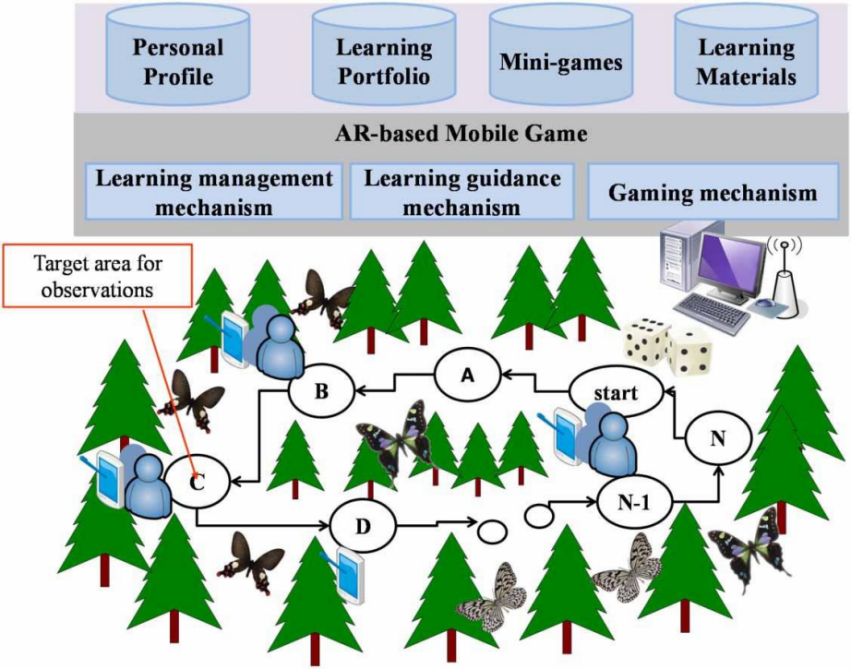
\includegraphics[scale=0.7]{figures/penelitian1.png}
    \caption{Augmented Reality Based Mobile Game System Structure.}
    \vspace{1em}
   \small Source: G.J. Hwang et al. (2016), Effects of an augmented reality-based educational game on students’ learning achievements and attitudes in real-world observations, \textit{Interactive Learning Environments}, pp. 4.
    \label{fig:my_label}
\end{figure}
This research has used a database to store assets and scenarios used. However, in this study, the application has not added 3D assets to present interactive learning so that it is more attractive to students' learning interests. This research has also not been applied to mobile devices with the iOS operating system so it can only be operated for Android OS, it also still uses QR code technology so it is necessary to develop a platform for markerless AR technology.

\begin{table}[h!]
\centering
\caption{Augmented Reality SDK Comparison. }
%\begin{adjustbox}{width=\columnwidth,center}
\resizebox{9cm}{!}{
\begin{tabular}{|c|c|c|c|c|c|c|c|c|c|} 
\toprule
\multicolumn{2}{|l|}{AR SDK}                                                          & \multirow{2}{*}{Vuvoria}                                                                  & \multirow{2}{*}{Metaio}                                                                          & \multirow{2}{*}{Wikitude}                                         & \multirow{2}{*}{ARToolkit}                                                              & \multirow{2}{*}{D'Fusion}                                                                & \multirow{2}{*}{ARmedia}                                          & \multirow{2}{*}{ARcore}                                                                                & \multirow{2}{*}{ARkit}                                           \\ 
\cline{1-2}
\multicolumn{2}{|c|}{Type}                                                            &                                                                                           &                                                                                                  &                                                                   &                                                                                         &                                                                                          &                                                                   &                                                                                                        &                                                                  \\ 
\hline
\multirow{6}{*}{Tracking} & Marker                                                    & \begin{tabular}[c]{@{}l@{}}Frame \\markers, \\image\\target, \\text \\target\end{tabular} & \begin{tabular}[c]{@{}l@{}}ID, \\picture \\and \\LLA \\marker, \\QR \\and \\Barcode\end{tabular} & \begin{tabular}[c]{@{}l@{}}Image,\\barcode\\tracking\end{tabular} & \begin{tabular}[c]{@{}l@{}}square \\marker, \\multiple \\marker \\tracking\end{tabular} & \begin{tabular}[c]{@{}l@{}}multiple\\marker,\\tracking,\\barcode \\tracking\end{tabular} & \begin{tabular}[c]{@{}l@{}}track \\fiducial \\marker\end{tabular} & \begin{tabular}[c]{@{}l@{}}motion\\tracking,\\build\\under-\\standing\\of the\\real world\end{tabular} & \begin{tabular}[c]{@{}l@{}}image,\\world\\tracking\end{tabular}  \\ 
\cline{2-10}
                          & GPS                                                       & N                                                                                         & Y                                                                                                & Y                                                                 & N                                                                                       & Y                                                                                        & Y                                                                 & Y                                                                                                      & Y                                                                \\ 
\cline{2-10}
                          & IMU                                                       & N                                                                                         & Y                                                                                                & Y                                                                 & N                                                                                       & Y                                                                                        & Y                                                                 & Y                                                                                                      & Y                                                                \\ 
\cline{2-10}
                          & Face                                                      & N                                                                                         & Y                                                                                                & N                                                                 & N                                                                                       & Y                                                                                        & N                                                                 & Y                                                                                                      & Y                                                                \\ 
\cline{2-10}
                          & \begin{tabular}[c]{@{}l@{}}Natural \\Feature\end{tabular} & Y                                                                                         & Y                                                                                                & Y                                                                 & Y                                                                                       & Y                                                                                        & Y                                                                 & Y                                                                                                      & Y                                                                \\ 
\cline{2-10}
                          & \begin{tabular}[c]{@{}l@{}}3D \\Object\end{tabular}       & Y                                                                                         & Y                                                                                                & N                                                                 & N                                                                                       & Y                                                                                        & Y                                                                 & Y                                                                                                      & Y                                                                \\
\bottomrule
\end{tabular}}
%\end{adjustbox}
\label{Tab:Table1}\\
\vspace{1em}
\small Source: Amin et al. (2015), Comparative  Study  of  Augmented  Reality  Sdk’s, \textit{International Journal on Computational Science}, pp. 25.
\end{table}

\begin{table}[h!]
\centering
\caption{Limitation AR SDK.}
\label{Tab:Table2}
\resizebox{7cm}{!}{
\begin{tabular}{|l|l|} 
\toprule
\multicolumn{2}{|l|}{Limitation}                                                                                                                                                                                              \\ 
\hline
Vuforia   & \begin{tabular}[c]{@{}l@{}}vuforia SDK for android doesn't expose any utility function \\to easily local a 3D model from any standart format. \\device database can only support 100 images targets\end{tabular}  \\ 
\hline
Metaio    & \begin{tabular}[c]{@{}l@{}}difficult to render complex 3D objects also limitation\\is associated with model size\end{tabular}                                                                                     \\ 
\hline
Wikitude  & \begin{tabular}[c]{@{}l@{}}doesn't track 3D model with limits is use to \\only 2D tracking. Target image to track need to \\be of solid colors to be recognizes\end{tabular}                                      \\ 
\hline
ARToolkit & \begin{tabular}[c]{@{}l@{}}less accuracy in tracking markers even when \\camera and marker are still. It itself doesn't \\support location based AR\end{tabular}                                                  \\ 
\hline
D'Fusion  & \begin{tabular}[c]{@{}l@{}}video file supported but audio associated\\with video can't be played\end{tabular}                                                                                                     \\ 
\hline
ARmedia   & doesn't support all type of textures for 3D objects                                                                                                                                                               \\ 
\hline
ARcore    & \begin{tabular}[c]{@{}l@{}}ARCore, on the other hand, will run on portable \\devices on a base of Android 7.0 Nougat and higher.\end{tabular}                                                                     \\ 
\hline
ARkit     & \begin{tabular}[c]{@{}l@{}}doesn't support android OS, need depth camera. \\ARKit is only compatible with iPads or \\iPhones on a base of iOS 11 and higher.\end{tabular}                                         \\ \hline
\end{tabular}}\\ 
{\vspace{1em}}
\small Source: Amin et al. (2015), Comparative  Study  of  Augmented  Reality  Sdk’s, \textit{International Journal on Computational Science}, halaman 23.
\end{table}



\include{Chapter3/chapter3}
%%%%%%%%%%%%%%%%%%%%%%%%%chapter4%%%%%%%%%%%%%%%%%%%%%%%%%%%
\chapter{EXPERIMENT AND ANALYSIS}
Uraian pada bab ini meliputi parameter eksperimen, karakteristik data, skenario ujicoba, tempat dan waktu eksperimen, spesifikasi peralatan ujicoba, cara penafsiran dan penyimpulan hasil tesis. Untuk tesis yang menggunakan metode kualitatif, dapat dijelaskan pendekatan yang digunakan, proses pengumpulan dan analisis informasi, proses penafsiran, dan penyimpulan hasil tesis. Analisis hasil eksperimen seharusnya dihubungkan kembali dengan permasalahan. Berikut contoh sistematika penulisan Bab 4.
\section{Experiment Parameter}
Disini penulis dapat membahas parameter eksperimen lebih terperinci. Deskripsi pembahasan seharusnya singkat, padat dan jelas, sehingga membuat pembaca memahami maksud Penulis yang tertuang dalam tulisan.
\section{TEMPAT UJICOBA}
Disini penulis dapat membahas tempat pelaksanaan ujicoba lebih terperinci. Deskripsi pembahasan seharusnya singkat, padat dan jelas, sehingga membuat pembaca memahami maksud penulis yang tertuang dalam tulisan.
\section{WAKTU UJICOBA}
Disini penulis dapat membahas waktu pelaksanaan ujicoba lebih terperinci. Deskripsi pembahasan seharusnya singkat, padat dan jelas, sehingga membuat pembaca memahami maksud penulis yang tertuang dalam tulisan.
\section{SPESIFIKASI PERALATAN UJICOBA}
Disini penulis dapat membahas spesifikasi peralatan lebih terperinci. Peralatan dapat berupa perangkat keras, perangkat lunak, piranti elektronik, gadget, dan lain-lain, yang berfungsi sebagai alat yang dipakai untuk percobaan. Deskripsi pembahasan seharusnya singkat, padat dan jelas, sehingga membuat pembaca memahami maksud penulis yang tertuang dalam tulisan.
\section{HASIL EKSPERIMEN}
Disini penulis dapat membahas hasil eksperimen lebih terperinci. Deskripsi pembahasan seharusnya singkat, padat dan jelas, sehingga membuat pembaca memahami maksud penulis yang tertuang dalam tulisan.
\section{ANALISIS HASIL EKSPERIMEN}
Disini penulis dapat membahas analisis hasil eksperimen lebih terperinci. Analisis hasil eksperimen seharusnya menjawab hipotesa bahwa solusi yang diajukan pada Tujuan dapat menyelesaikan permasalahan. Deskripsi pembahasan seharusnya singkat, padat dan jelas, sehingga membuat pembaca memahami maksud penulis yang tertuang dalam tulisan. 

\chapter{CONCLUSION}
Bab 5 memuat penjelasan ringkas dari apa yang telah ditulis dari Bab 1 sampai Bab 4. Bab Penutup ini memuat 2 bagian penting, yaitu (1) Kesimpulan, dan (2) Saran.
\section{KESIMPULAN}
Disini berikan kesimpulan terhadap Problem dan tingkat urgensi, solusi yang penulis tawarkan, orisinalitas pada tesis ini, desain sistem, eksperimen dan kinerja sistem terhadap permasalahan.
\section{SARAN}
Solusi yang penulis tawarkan pasti mempunyai sisi-sisi keterbatasan. Berikanlah suatu saran terhadap keterbatasan tersebut untuk pengembangan dan peningkatan solusi dalam menjawab permasalahan.

%\include{Chapter6/chapter6}
%\include{Chapter7/chapter7}



% ********************************** Back Matter *******************************
% Backmatter should be commented out, if you are using appendices after References
%\backmatter

% ********************************** Bibliography ******************************
\begin{spacing}{0.9}

% To use the conventional natbib style referencing
% Bibliography style previews: http://nodonn.tipido.net/bibstyle.php
% Reference styles: http://sites.stat.psu.edu/~surajit/present/bib.htm

\bibliographystyle{plainnat}
%\bibliographystyle{unsrt} % Use for unsorted references  
%\bibliographystyle{plainnat} % use this to have URLs listed in References
\cleardoublepage
% \bibliography{References/references} % Path to your References.bib file
\bibliography{reference.bib}


% If you would like to use BibLaTeX for your references, pass `custombib' as
% an option in the document class. The location of 'reference.bib' should be
% specified in the preamble.tex file in the custombib section.
% Comment out the lines related to natbib above and uncomment the following line.

%\printbibliography[heading=bibintoc, title={References}]


\end{spacing}

% ********************************** Appendices ********************************

\begin{appendices} % Using appendices environment for more functunality

\newpage
\chapter{JUUDL LAMPIRAN}
Lampiran berisi informasi yang menunjang bahasan dalam Buku Tesis, seperti data yang cukup banyak, datasheet, pembuktian matematis, dan lain-lain. Lampiran dapat berupa tabel, gambar, worksheet, foto, dan lain-lain. Jika lembaran lampiran lebih besar dari batas ukuran buku tesis, lembar lampiran dapat dilipat sehingga tidak melebihi batas ukuran buku.
\newpage
\chapter{JUUDL LAMPIRAN}
Lampiran berisi informasi yang menunjang bahasan dalam Buku Tesis, seperti data yang cukup banyak, datasheet, pembuktian matematis, dan lain-lain. Lampiran dapat berupa tabel, gambar, worksheet, foto, dan lain-lain. Jika lembaran lampiran lebih besar dari batas ukuran buku tesis, lembar lampiran dapat dilipat sehingga tidak melebihi batas ukuran buku.



\end{appendices}

% *************************************** Index ********************************
\printthesisindex % If index is present

\end{document}
